We run the experimental process from section~\ref{sec:rational} on the
sampled debugging scenarios from section~\ref{sec:sample} using a machine with two Intel Xeon Gold 6258R processors (28 doubly-threaded cores each) and 500GB of memory.
Each debugging scenario had a timeout limit of 4 minutes and a
memory limit of 6GB. The complete experiment required
over 30,000 hours of compute hours.


\begin{wrapfigure}{r}{.40\textwidth}
  \centering
  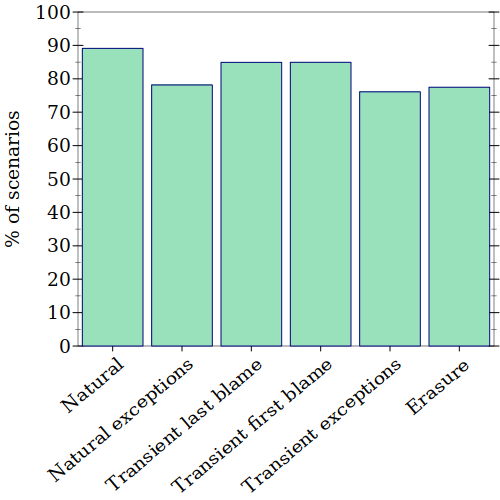
\includegraphics[width=0.40\textwidth]{./plots/success-bars}
  \caption{Success baselines: The estimated percentage of scenarios for which each mode succeeds in locating the bug.
  The upper bound of error margin is 0.02\%.
  }
  \label{fig:success-bars}
\end{wrapfigure}

\begin{figure}
  \centering
  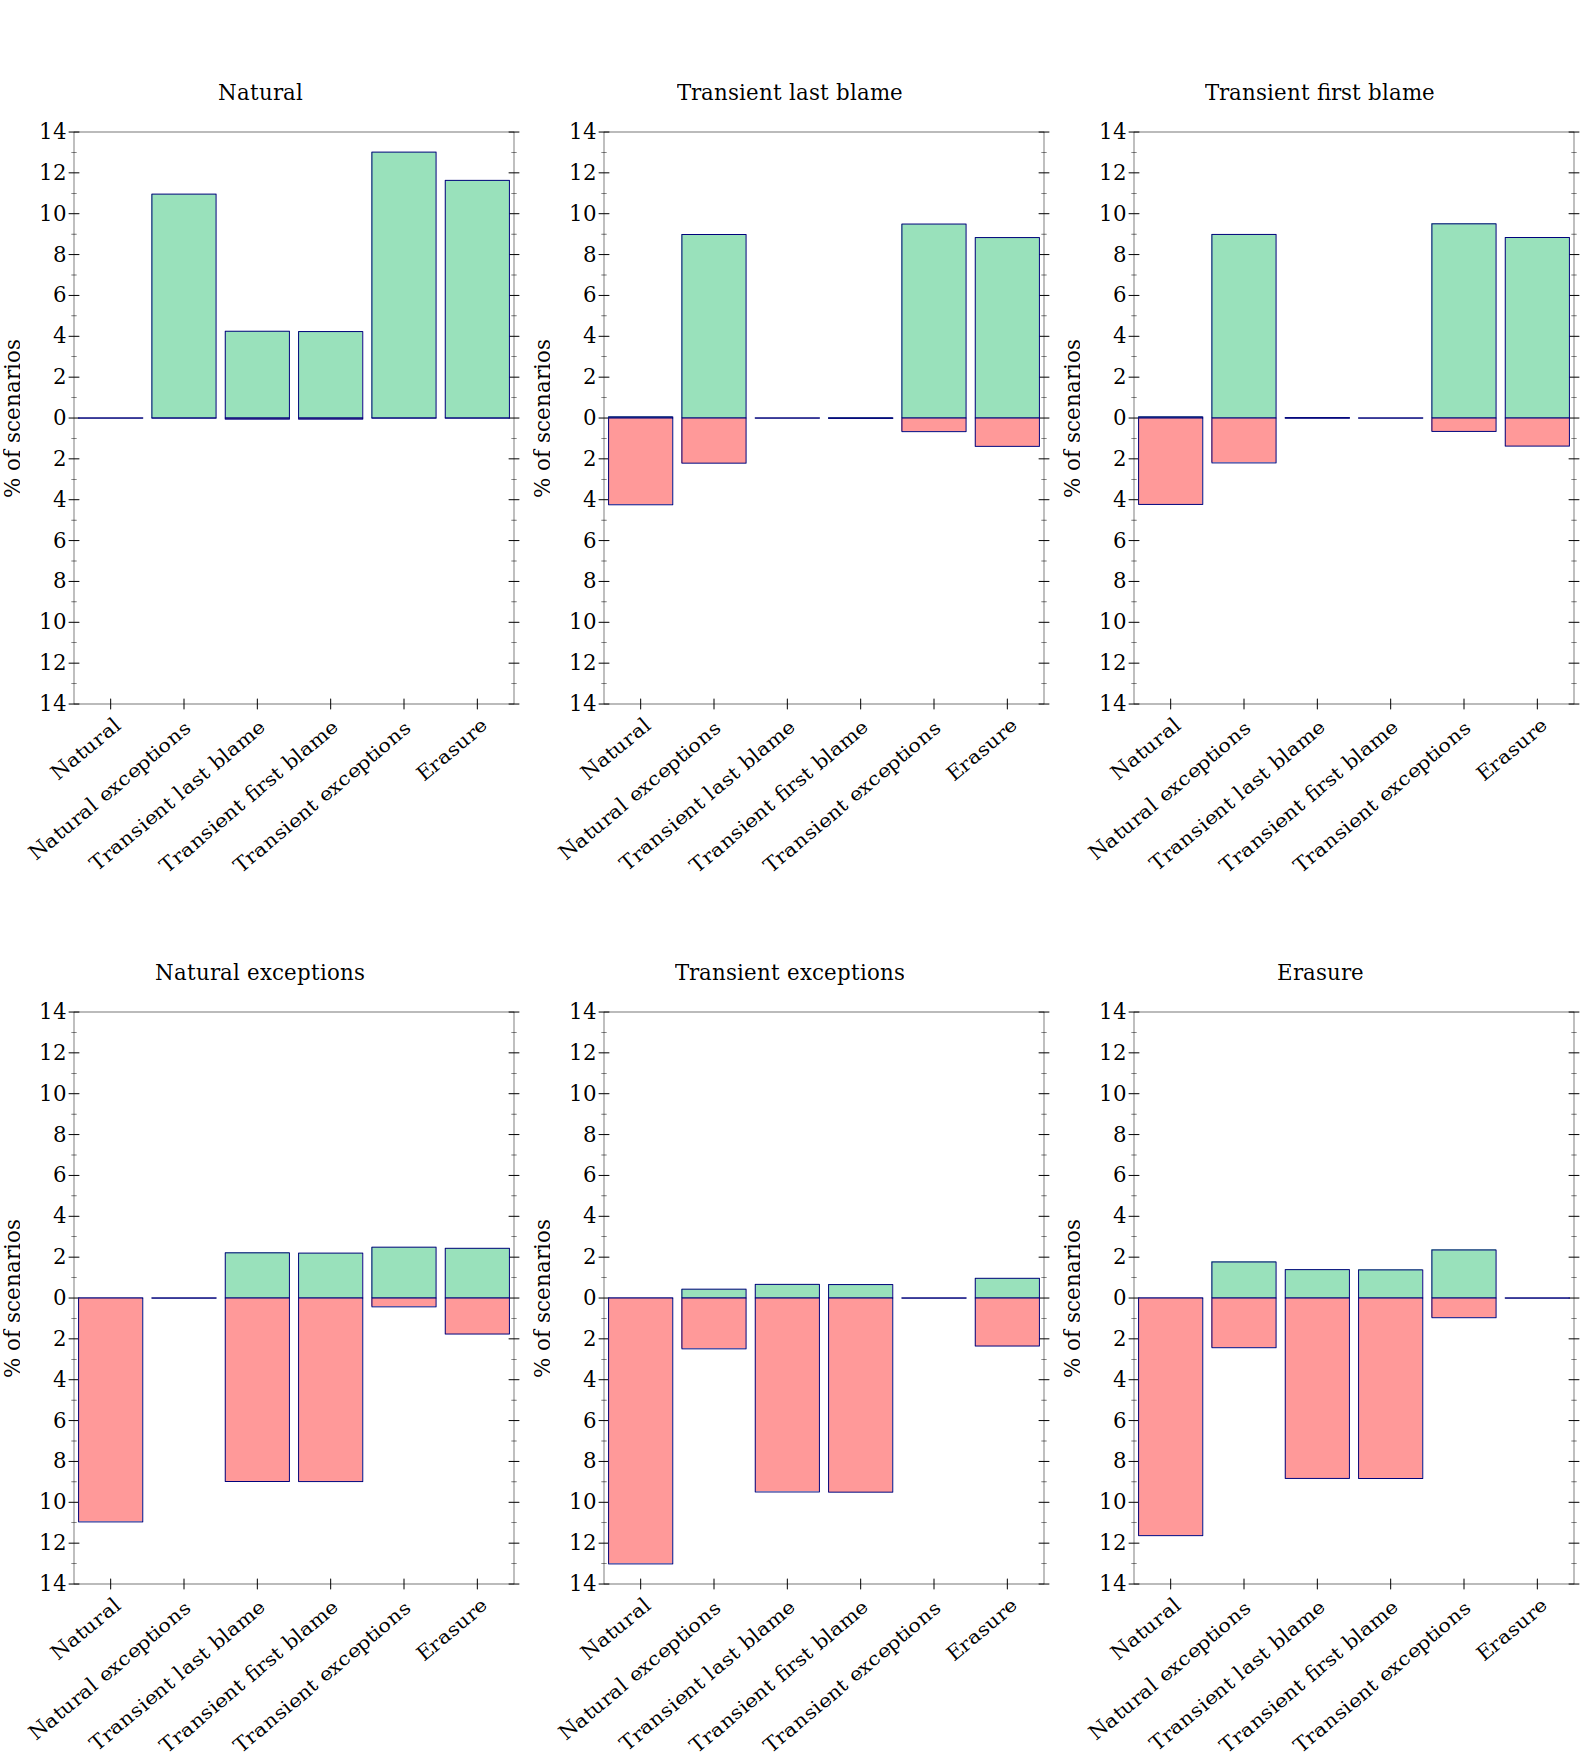
\includegraphics[width=\textwidth]{./plots/avo-bars}
  \caption{Usefulness comparisons: Each plot depicts a head-to-head comparison of the entitled mode against every other mode.
  The portion above 0 (in green) is the estimated percentage of scenarios where the entitled mode is more useful than each of the other modes.
  The portion below 0 (in red) is the estimated percentage of scenarios with the inverse situation.
  The upper bound of error margin is 0.02\%.
  }
  \label{fig:avo-bars}
\end{figure}

\begin{figure}
  \centering
  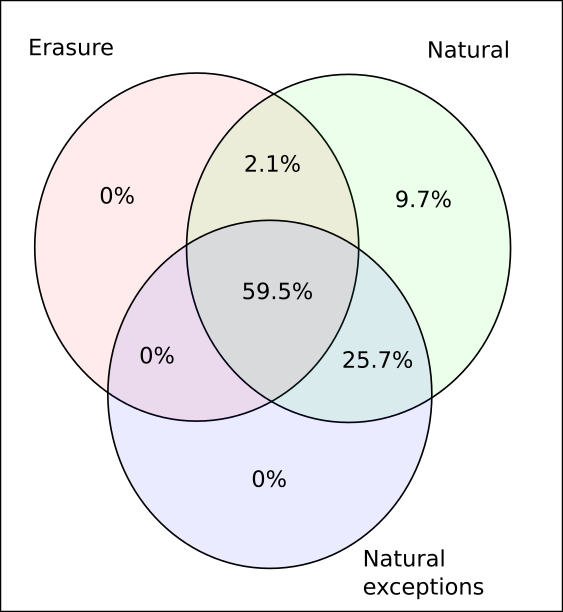
\includegraphics[width=0.32\textwidth]{./plots/TR-TR-stack-first-venn}
  \hfill
  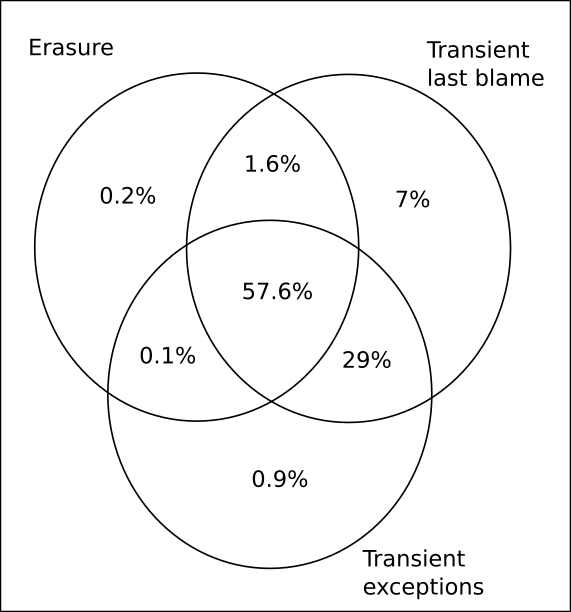
\includegraphics[width=0.32\textwidth]{./plots/transient-newest-transient-stack-first-venn}
  \hfill
  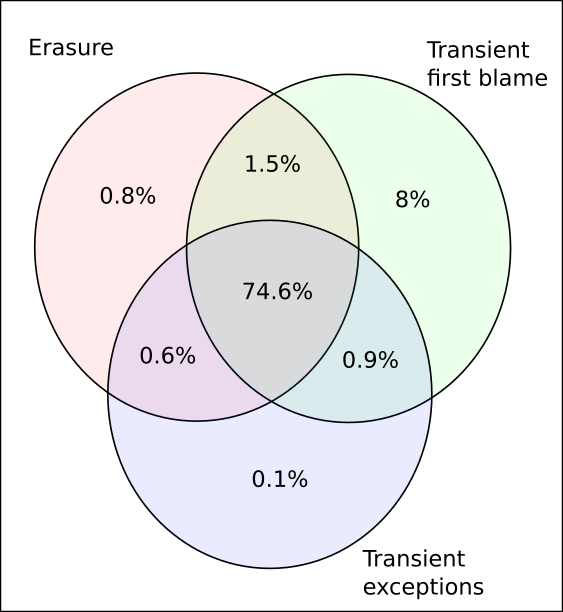
\includegraphics[width=0.32\textwidth]{./plots/transient-oldest-transient-stack-first-venn}

  \caption{Blame usefulness analysis: Each diagram shows the breakdown of how three modes' successful scenarios overlap.
  The percentage of scenarios covered by each circle are proportions for which the corresponding mode succeeds.
  For example, in the breakdown of Natural, all three modes succeed on the same scenario 57.3\% of the time, only Natural and Natural exceptions succeed on 29.1\% of the scenarios, only Natural and Erasure succeed on 2.1\%, and Natural alone succeeds on 9\%.
  The upper bound of error margin is 0.02\%.
  }
  \label{fig:success-venns}
\end{figure}


Figure~\ref{fig:success-bars} summarizes the overall success rates of every mode.
The success rates illustrate a few points that underly the rest of our analysis.
The first notable piece of information from
this figure is that every mode has failed debugging scenarios, not just
Erasure. This should
not come as a surprise to the astute
reader. After all, as we
discuss above, some modes are more successful than others in certain
scenarios. Indeed any mode can fail if running a scenario results in an
exception and the exception carries no useful information about which
module the programmer should type next, e.g., because the stack trace 
does not contain frames from any module of the program, or only typed modules. This situation
can happen several steps along a blame trail or even immediately (figure~\ref{fig:effort-table} dives into this below).

While most failures to debug scenarios follow the above pattern, a few do not.
Breaking down the reasons for failure for Natural blame (1748 in total)
reveals an additional cause. For a small set of
debugging scenarios (40), Natural produces a run time type error
blaming a non-buggy already typed
component. We tracked down all these cases to known open issues with Typed
Racket and class contracts. 

In Transient, similar to Natural,
most failures are due to unhelpful exception information (1851 for both
Transient first and last blame).  
However, Transient also has a substantial
number of failures because scenarios hit the time and memory
limits of our experiment (~ 770 scenarios).  Additionally, there are nearly a 1000 cases where
Transient reports an empty blame set which leaves the rational programmer
without hints about how to proceed.
In~\ref{sec:threat:transient}, we discuss how both of these causes of
failure for Transient affect our experiment. 

The second key observation from figure~\ref{fig:success-bars} is that the modes that use blame all outperform those that do not.
In particular, Natural and both of Transient's blame modes succeed in around 95\% of our scenarios, while their corresponding exception modes succeed in around 85\% of them and Erasure succeeds in only 60\% of them.
The only exception is that the Random programmer always succeeds;
this reflects the fact that every scenario has finitely many modules and this mode can never get stuck.


Figure~\ref{fig:avo-bars} depicts a head-to-head comparison of every mode's performance against every other mode, helping to answer the four questions from section~\ref{sub:experiment}.
Each plot shows a breakdown of the proportion of scenarios where one mode performs better or worse than each other mode.
In particular, each bar above zero represents the proportion where the plot's entitled mode succeeds and the mode on the x-axis fails; the correspnding bar below zero represents the proportion of the opposite case.
For example, the plot titled ``Natural'' shows that Natural outperforms Natural exceptions in about 10\% of the scenarios, and the inverse (Natural performs wrse than Natural exceptions) never happens.
Similarly, the plot titled ``Transient last blame'' shows that Transient last blame outperforms Natural exceptions about in abut 10\% of the scenarios, but conversely it performs worse than Natural exceptions in about 2\% of the scenarios.

Figure~\ref{fig:avo-bars} shows that the answers for questions $Q_1$ to $Q_3$ are all positive.
In all three semantics, blame modes outperform their corresponding exception mode (by around 10\% for each one).
The Natural exceptions mode is never more useful than Natural blame, and  Transient
exceptions are more useful than Transient first and Transient last blame
in a small percentage (about 2\%) of the scenarios. 

Figure~\ref{fig:avo-bars} also provides answers to $Q_*$.
Blame for all three semantics is significantly
more useful than Erasure exceptions (by around 30\%). Natural blame is
more useful than both versions of Transient blame by a small percentage;
in about 4\% of scenarios Natural blame is more useful while in about 1.5\% of the
scenarios Transient blame is more useful. The Transient first and
Transient last blame are practically indistinguishable. Finally, there is
no clear winner between Natural exceptions and Transient exceptions
despite the theoretically advantageous additional checks of the Natural
semantics.

\begin{figure}
  \centering
  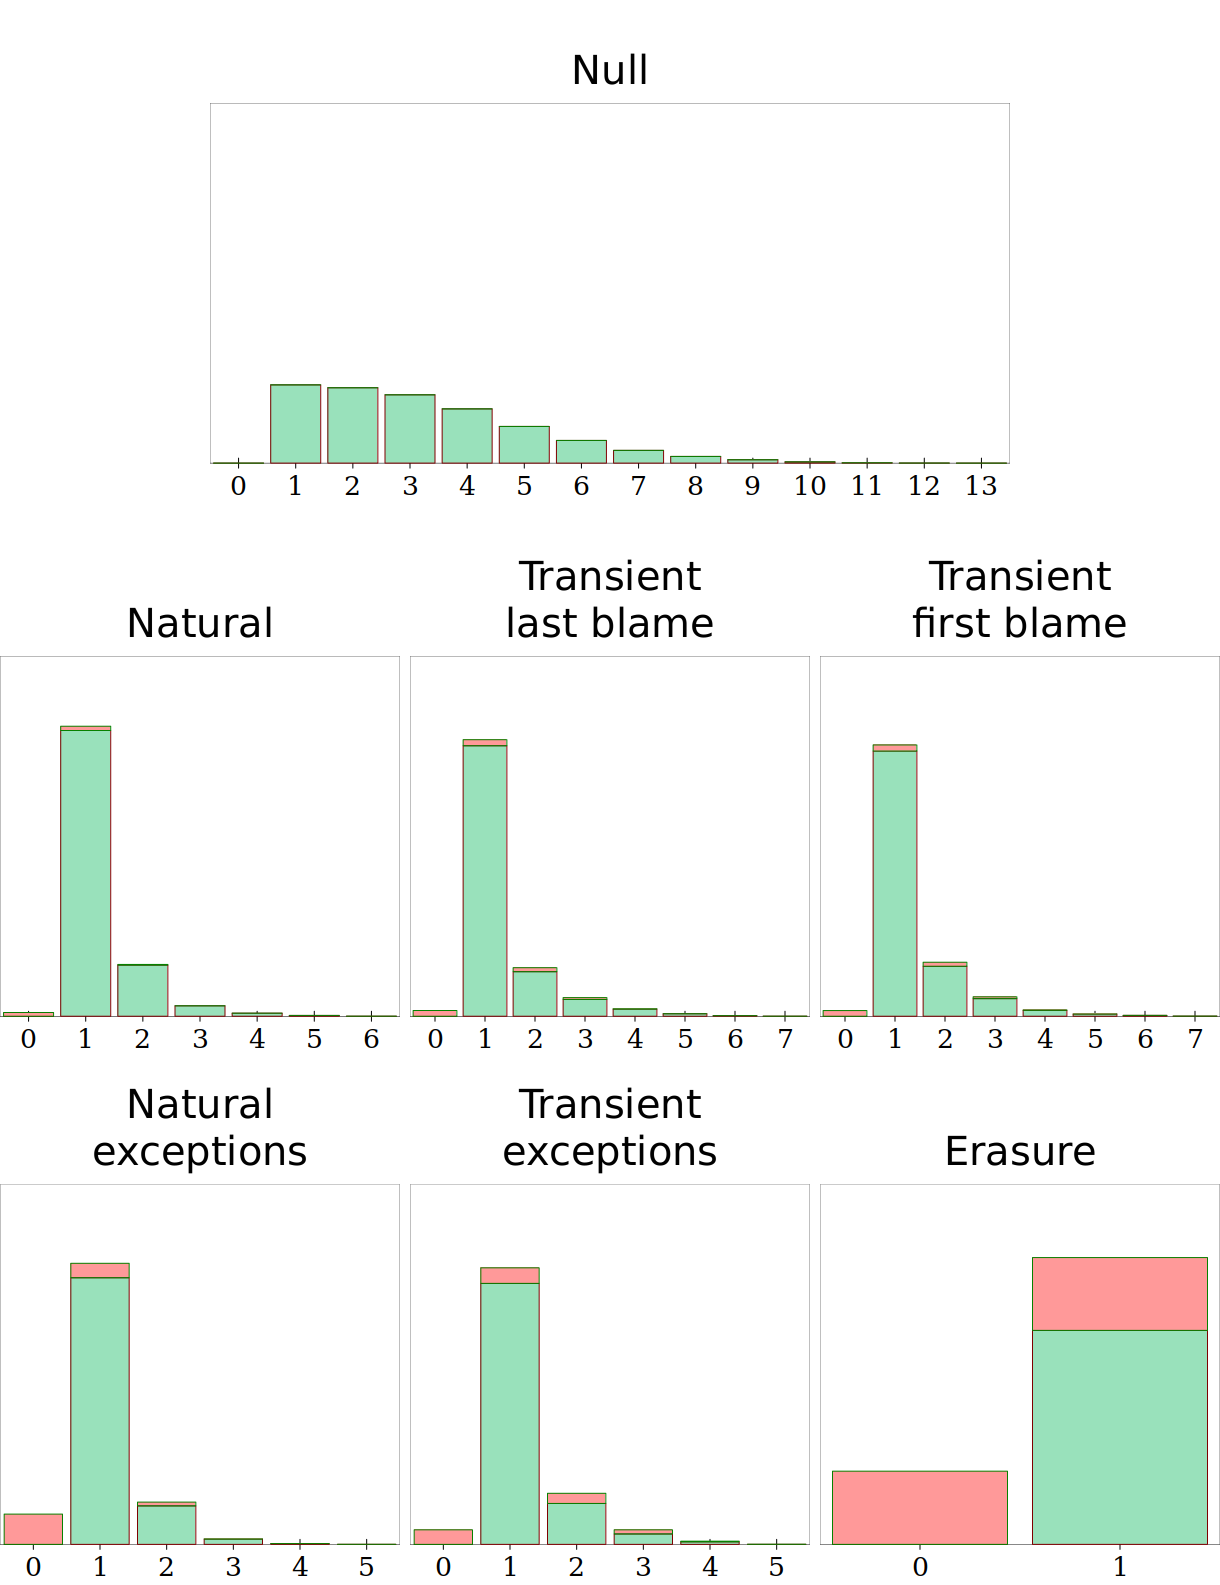
\includegraphics[width=\textwidth]{./plots/bt-lengths-table}
  \caption{Programmer effort: Each plot depicts the distribution of trail
  lengths for a given mode across all benchmarks.}
  \label{fig:effort-table}
\end{figure}

\begin{figure}
  \centering
  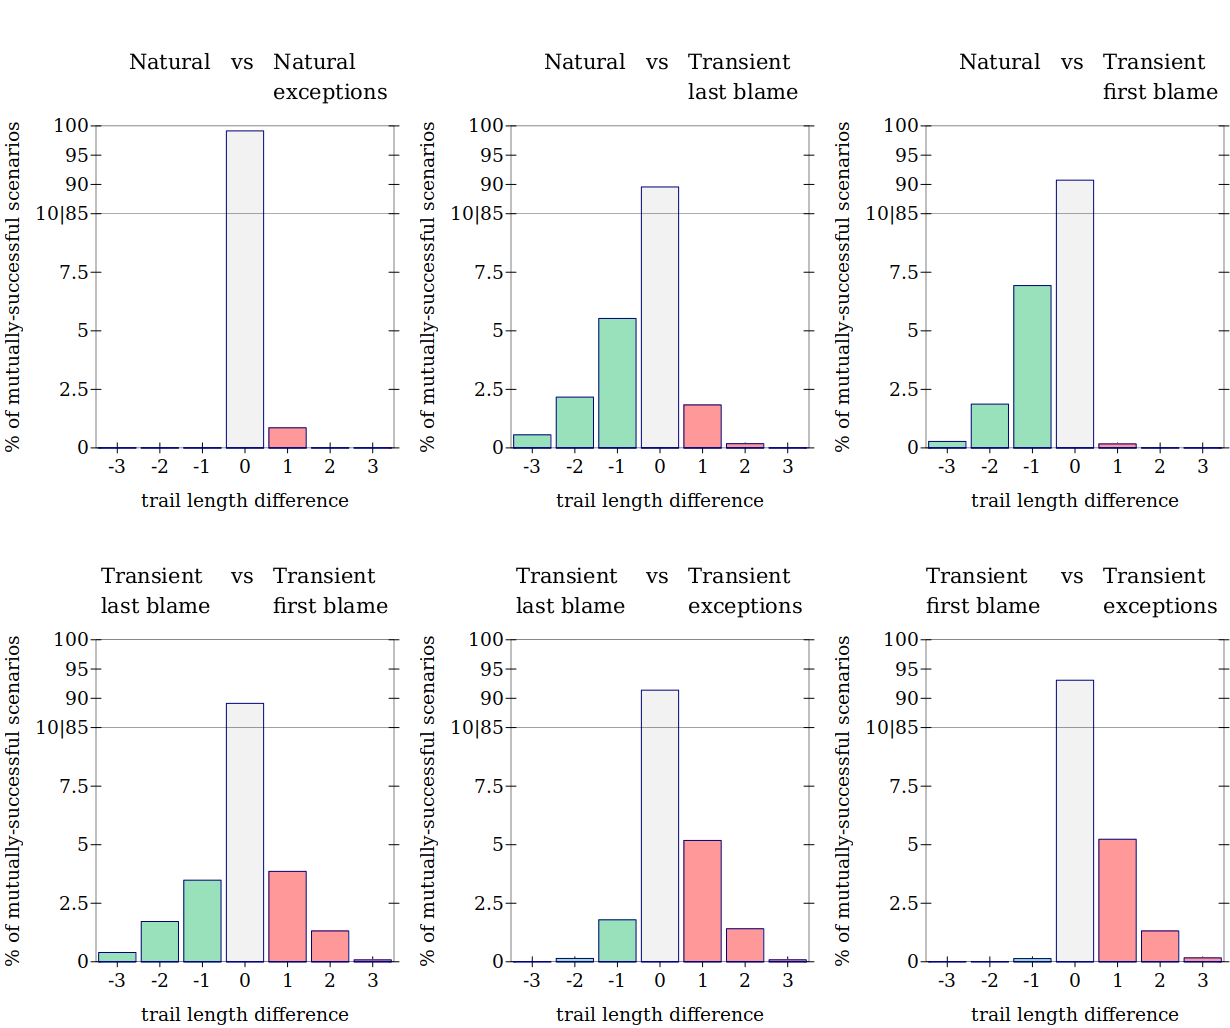
\includegraphics[width=\textwidth]{./plots/bt-length-comparisons}
  \caption{Effort comparisons: Each plot depicts the distribution of scenarios with trail length differences ranging from -3 to 3.
  A negative difference means that the first mode's trail is three steps shorter than the second mode's trail for the same scenario, and a positive difference is the reverse.
  Only scenarios where both modes succeed are considered.
  The 10|85 on the y-axis indicates that the axis is truncated between 10 and 85\%.}
  \label{fig:effort-comparisons}
\end{figure}

In order to better understand questions $Q_1$ to $Q_3$, figure~\ref{fig:success-venns} depicts a breakdown of the success of each semantics in comparison to Erasure.
Specifically, the figure shows one Venn diagram per mode of the rational programmer that uses blame.
Each diagram breaks breaks down the overlap in the success of the blame mode, its corresponding exception mode, and Erasure.
For example, in the breakdown of Natural, the diagram shows that all three modes succeed on the same scenario 57.3\% of the time, only Natural and Natural exceptions succeed on 29.1\% of the scenarios, only Natural and Erasure succeed on 2.1\%, and Natural alone succeeds on 9\%.
This analysis highlights the success tradeoffs each semantics offers against Erasure, with and without blame, to answer questions about the tradeoffs in choosing to use blame or just exceptions for each semantics.
For instance, the breakdown of Natural clearly illustrates that if choosing between Natural blame, Natural exceptions, and Erasure, Natural blame is the absolutely most successful: all of the successes of the other two modes are subsets of Natural's successful scenarios.
On the other hand, Transient's blame modes are similar but not so clear-cut.


Turning to programmer effort, figure~\ref{fig:effort-table} shows the distribution of blame trail lengths
for our sample of interesting debugging scenarios. Unlike the usefulness
comparisons above, these proportions do not generalize to a representation of the full population.
Still, as we discuss in section~\ref{subsec:effort}, they provide an
alternative view of the workings of the rational programmer. 

There are
two immediate take-aways from the figure. First, the effort for successfully
debugging interesting scenarios (in green) for the random mode of the
rational programmer follows  a normal distribution, as expected.\footnote{The
random mode distribution is indistinguishable for all three semantics and thus the figure~\ref{fig:effort-table} 
only shows one plot.} In contrast, in the other modes, successful effort coalesces at
the left side of the plot, meaning that in most cases the programmer needs
to type a single component to debug a scenario. 

A second point of interest is that the exceptions of
the Erasure semantics either help the rational programmer immediately or 
the rational programmer fails to debug a scenario altogether (in red).
This is expected; no matter how many type annotations the programmer
adds to an Erasure program, if the type checker doesn't reject the
program, running the program always produces the same outcome. Thus an
exception from the runtime has to point to the buggy module with
the first try. Otherwise the rational programmer types an irrelevant
module, runs the program again and the exception points again to the
already typed module. 

Figure~\ref{fig:effort-comparisons} provides head-to-head comparisons of effort.
To directly compare effort between modes, we compute the difference in trail length between two modes for all scenarios where they both succeed.
Hence, each plot in the figure shows the distribution of scenarios with length differences ranging from -3 (the first mode's trail is 3 steps shorter than the second) to 3 (the first mode's trail is 3 steps longer than the second).
The figure offers several insights about the comparative effort for each mode that complement the insights about comparitive success from figure~\ref{fig:avo-bars}.
First, Natural blame never produces shorter trails than Natural exceptions, and sometimes (albeit rarely) produces slightly longer ones.
Second, Natural relatively often (around 10\% of the scenarios) produces shorter trails than both Transient blame modes, and they are sometimes significantly shorter.
Third, Transient last blame often produces shorter trails than Transient first blame, which is a particularly interesting distinction in light of their nearly undistinguishable success rates.
Finally, Transient's blame modes also share the characteristic with Natural that blame sometimes produces longer trails than their corresponding exception modes.

